\documentclass[12pt]{article}

\usepackage[spanish]{babel}
\usepackage[utf8]{inputenc}
\usepackage{graphicx}
\usepackage{geometry}
\usepackage{xcolor}
\usepackage{fancyhdr}
\usepackage{lastpage}
\usepackage{pdfpages}
\usepackage{listings}

\geometry{top=25mm,left=15mm,right=15mm,a4paper}

\pagestyle{fancy}
\fancyhf{}
\lhead{Seminario de Ciencias de la Computación A}
\cfoot{Página \thepage\ de \pageref{LastPage}}

\graphicspath{./}

\begin{document}
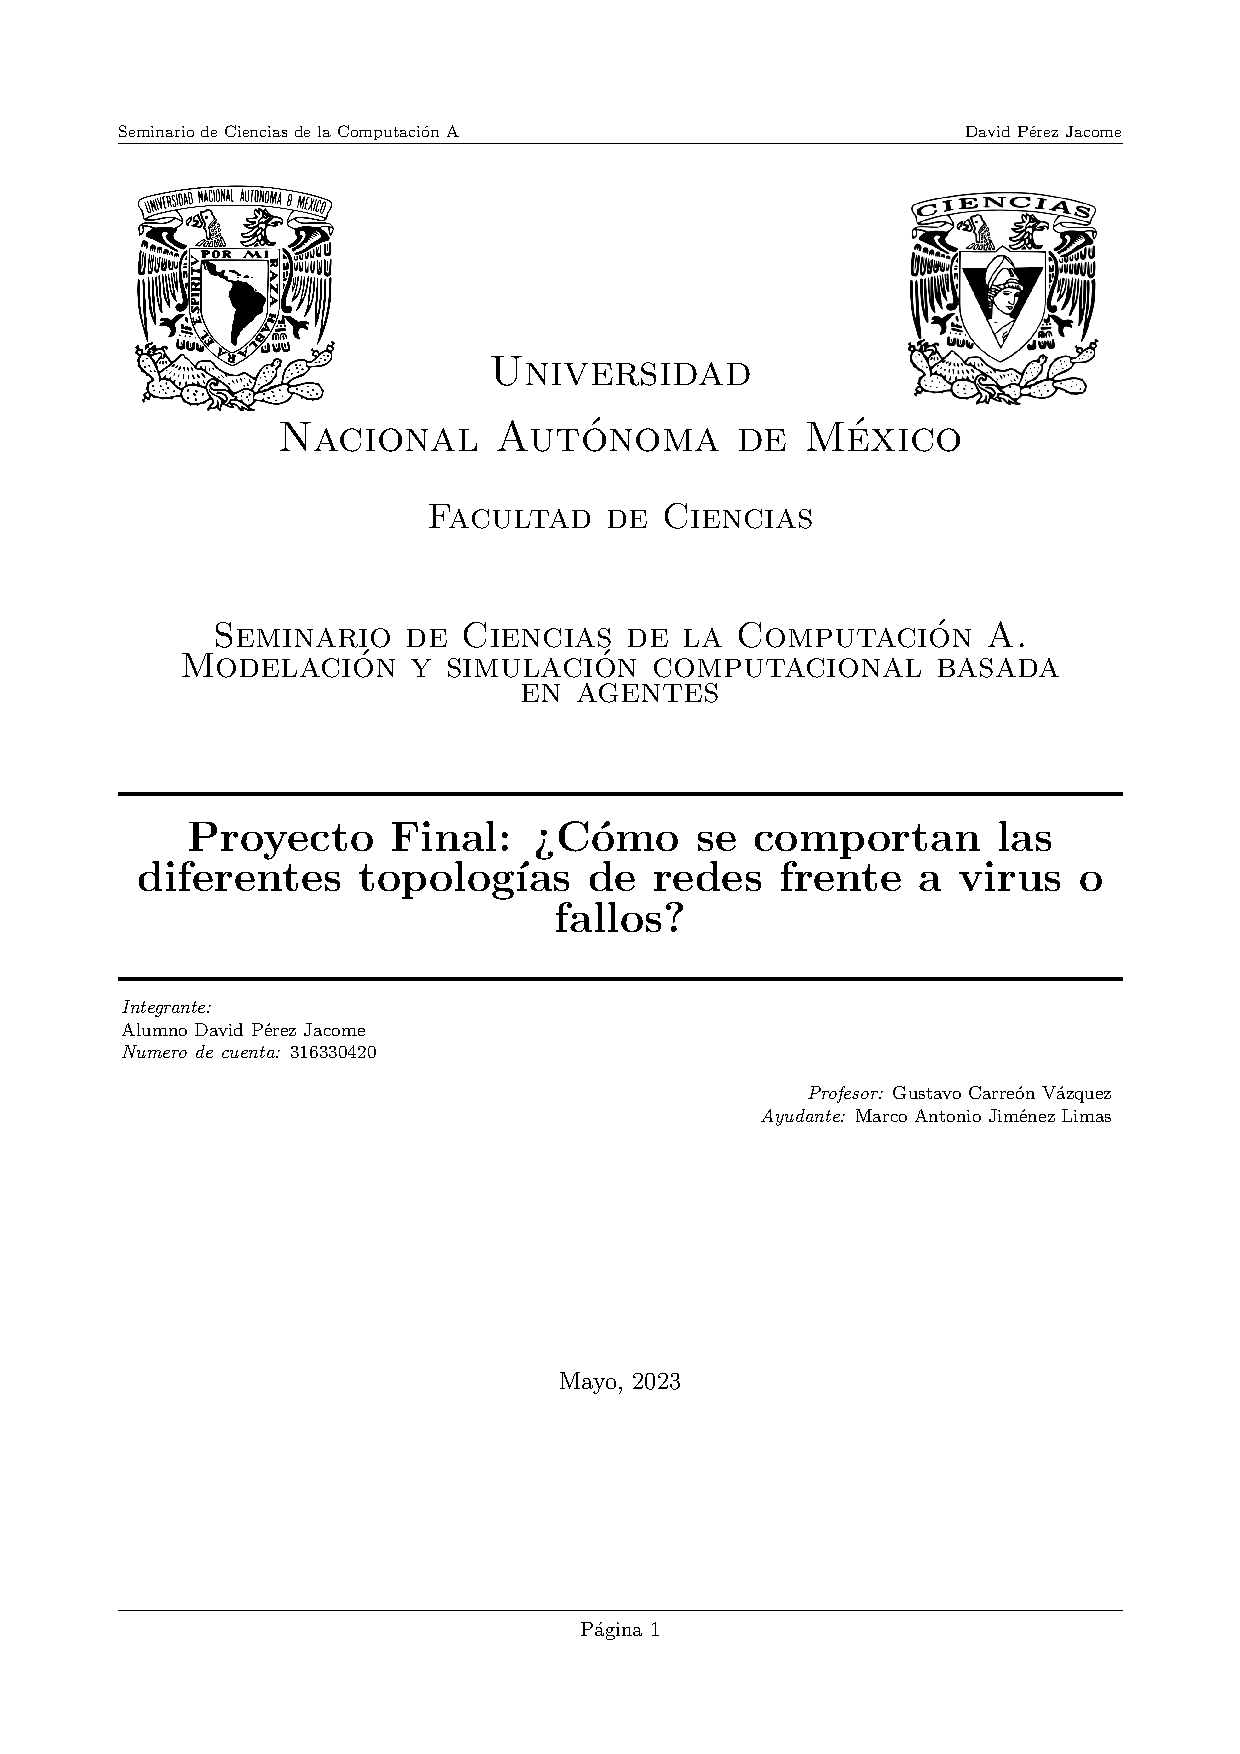
\includepdf{Portada.pdf}
{\color{red} \section*{Proyecto Final: ¿Cómo se comportan las diferentes topologías de redes frente a virus o fallos?.}}
\vspace{2em}

{\color{blue} \subsection*{1- INTRODUCCIÓN.}}
\vspace{1em}

¿Cómo se comportan las diferentes topologías de redes frente a virus o fallos?, esta es la pregunta a la que a lo largo de este trabajo nos vamos a dedicar a responder.
A lo largo del curso de Modelación Basada en Agentes hemos ido aprendiendo diversas aplicaciones y simulaciones del mundo real en las que podemos "modelar" y mostrar el como es el comportamiento de algún fenomeno
ya sea fisico o en este caso computacional, en este trabajo abordaremos principalmente la problematica de modelar una estructura de red, pero para ello debemos tener presente que es un sistema de redes, que en pocas palabras una red de ordenadores se refiere a dispositivos de computación 
interconectados que pueden intercambiar datos y compartir recursos entre sí. 
Los dispositivos de la red utilizan un sistema de reglas, llamados protocolos de comunicaciones, para transmitir información a través de tecnologías físicas o inalámbricas.















{\color{blue} \subsection*{2- PLANTEAMIENTO.}}
\vspace{1em}


{\color{blue} \subsection*{3- DESARROLLO.}}
\vspace{1em}

{\color{blue} \subsection*{4- RESULTADOS.}}
\vspace{1em}

{\color{blue} \subsection*{5- CONCLUSIONES Y REFLEXIONES.}}
\vspace{1em}

{\color{blue} \subsection*{6- BIBLIOGRAFIA.}}
\vspace{1em}

\begin{thebibliography}{99}
    \bibitem{1}
    Amazon Web Services. (s.f.). What is Computer Networking? Recuperado de https://aws.amazon.com/es/what-is/computer-networking/
\end{thebibliography}


\end{document}